%% В этот файл не предполагается вносить изменения

% В этом файле следует указать информацию о себе
% и выполняемой работе.

\documentclass [fontsize=14pt, paper=a4, pagesize, DIV=calc]%
{scrartcl}
% ВНИМАНИЕ! Для использования глав поменять
% scrartcl на scrreprt

% Здесь ничего не менять
\usepackage [T2A] {fontenc}   % Кириллица в PDF файле
\usepackage [utf8] {inputenc} % Кодировка текста: utf-8
\usepackage [russian] {babel} % Переносы, лигатуры

%%%%%%%%%%%%%%%%%%%%%%%%%%%%%%%%%%%%%%%%%%%%%%%%%%%%%%%%%%%%%%%%%%%%%%%%
% Создание макроса управления элементами, специфичными
% для вида работы (курс., бак., маг.)
% Здесь ничего не менять:
\usepackage{ifthen}
\newcounter{worktype}
\newcommand{\typeOfWork}[1]
{
	\setcounter{worktype}{#1}
}

% ВНИМАНИЕ!
% Укажите тип работы: 0 - курсовая, 1 - бак., 2 - маг.,
% 3 - бакалаврская с главами.
\typeOfWork{1}
% Считается, что курсовая и бак. бьются на разделы (section) и
% подразделы (subsection), а маг. — на главы (chapter), разделы и
%  подразделы. Если хочется,
% чтобы бак. была с главами (например, если она большая),
% надо выбрать опцию 3.

% Если при выборе 2 или 3 вы забудете поменять класс
% документа на scrreprt (см. выше, в самом начале),
% то получите ошибку:
% ./aux/appearance.tex:52: Package scrbase Error: unknown option ` chapterprefix=

%%%%%%%%%%%%%%%%%%%%%%%%%%%%%%%%%%%%%%%%%%%%%%%%%%%%%%%%%%%%%%%%%%%%%%%%
% Информация об авторе и работе для титульной страницы

\usepackage {titling}

% Имя автора в именительном падеже (для маг.)
\newcommand {\me}{%
И.\,И.~Иванов%
}

% Имя автора в родительном падеже (для курсовой и бак.)
\newcommand {\byme}{%
В.\,М.~Ложкиной%
}

% Научный руководитель
\newcommand{\supervisor}%
{старший преподаватель кафедры информатики и вычислительного эксперимента В.\,Н.~Брагилевский}

% идентифицируем пол (только для курсовой и бак.)
\newcommand{\bystudent}{
Студентки % Для курсовой: с большой буквы
}

% Год публикации
\date{2018}

% Название работы
\title{Реализация распределённого отказоустойчивого пространства кортежей средствами языка~Python}

% Кафедра
%

\newcommand {\direction} {%
Направление подготовки\\01.\ifthenelse{\value{worktype} = 2}{04}{03}.02 ---
Прикладная математика\\и информатика%
}

%%%%%%%%%%%%%%%%%%%%%%%%%%%%%%%%%%%%%%%%%%%%%%%%%%%%%%%%%%%%%%%%%%%%%%%%
% Другие настраиваемые элементы текста

% Листинги с исходным кодом программ: укажите язык программирования
\usepackage{listings}
\lstset{
    language=Python,%  Язык указать здесь
    basicstyle=\small\ttfamily,
    breaklines=true,%
    showstringspaces=false%
    inputencoding=utf8x%
}
% полный список языков, поддерживаемых данным пакетом, есть,
% например, здесь (стр. 13):
% ftp://ftp.tex.ac.uk/tex-archive/macros/latex/contrib/listings/listings.pdf

% Нумерация списков: можно при необходимести
% изменять вид нумерации (например, добавлять правую скобку).
% По умолчанию буду списки вида:
% 1.
% 2.
% Изменять вид нумерации можно в начале нумерации:
% \begin{enumerate}[1)] (В квадратных скобках указан желаемый вид)
\usepackage[shortlabels]{enumitem}
                    \setlist[enumerate, 1]{1.}

% Гиперссылки: настройте внешний вид ссылок
\usepackage%
[pdftex,unicode,pdfborder={0 0 0},draft=false,%backref=page,
    hidelinks, % убрать, если хочется видеть ссылки: это
               % удобно в PDF файле, но не должно появиться на печати
    bookmarks=true,bookmarksnumbered=false,bookmarksopen=false]%
{hyperref}


\usepackage {amsmath}      % Больше математики
\usepackage {amssymb}
\usepackage {textcase}     % Преобразование к верхнему регистру
\usepackage {indentfirst}  % Красная строка первого абзаца в разделе

\usepackage {fancyvrb}     % Листинги: определяем своё окружение Verb
\DefineVerbatimEnvironment% с уменьшенным шрифтом
	{Verb}{Verbatim}
	{fontsize=\small}

% Вставка рисунков
\usepackage {graphicx}

% Общее оформление
% ----------------------------------------------------------------
% Настройка внешнего вида

%%% Шрифты

% если закомментировать всё — консервативная гарнитура Computer Modern
\usepackage{paratype} % профессиональные свободные шрифты
%\usepackage {droid}  % неплохие свободные шрифты от Google
%\usepackage{mathptmx}
%\usepackage {mmasym}
%\usepackage {psfonts}
%\usepackage{lmodern}
%var1: lh additions for bold concrete fonts
%\usepackage{lh-t2axccr}
%var2: the package below could be covered with fd-files
%\usepackage{lh-t2accr}
%\usepackage {pscyr}

% Геометрия текста

\usepackage{setspace}       % Межстрочный интервал
\onehalfspacing

\newlength\MyIndent
\setlength\MyIndent{1.25cm}
\setlength{\parindent}{\MyIndent} % Абзацный отступ
\frenchspacing            % Отключение лишних отступов после точек
\KOMAoptions{%
    DIV=calc,         % Пересчёт геометрии
    numbers=endperiod % точки после номеров разделов
}

                            % Консервативный вариант:
%\usepackage                % ручное задание геометрии
%[%                         % (не рекомендуется в проф. типографии)
%  margin = 2.5cm,
  %includefoot,
  %footskip = 1cm
%] %
%  {geometry}

%%% Заголовки


\ifthenelse{{\value{worktype} > 1}}{%
  \KOMAoptions{%
      headings=normal,   % размеры заголовков поменьше стандартных
      chapterprefix=true,% Печатать слово Глава
      appendixprefix=true% Печатать слово Приложение
  }
}{% Печатать слово Приложение даже если нет глав
  \newcommand*{\appendixmore}{%
    \renewcommand*{\sectionformat}{%
    \appendixname~\thesection\autodot\enskip}
    \renewcommand*{\sectionmarkformat}{%
      \appendixname~\thesection\autodot\enskip}
  }
}

% шрифт для оформления глав и названия содержания
\newcommand{\SuperFont}{\Large\sffamily\bfseries}

% Заголовок главы
\ifthenelse{\value{worktype} > 1}{%
\renewcommand{\SuperFont}{\Large\normalfont\sffamily}
\newcommand{\CentSuperFont}{\centering\SuperFont}
\usepackage{fncychap}
\ChNameVar{\SuperFont}
\ChNumVar{\CentSuperFont}
\ChTitleVar{\CentSuperFont}
\ChNameUpperCase
\ChTitleUpperCase
}

% Заголовок (под)раздела с абзацного отступа
\addtokomafont{sectioning}{\hspace{\MyIndent}}

\renewcommand*{\captionformat}{~---~}
\renewcommand*{\figureformat}{Рисунок~\thefigure}

% Плавающие листинги
\usepackage{float}
\floatstyle{ruled}
\floatname{ListingEnv}{Листинг}
\newfloat{ListingEnv}{htbp}{lol}[section]

% точка после номера листинга
\makeatletter
\renewcommand\floatc@ruled[2]{{\@fs@cfont #1.} #2\par}
\makeatother


%%% Оглавление
\usepackage{tocloft}

% шрифт и положение заголовка
\ifthenelse{\value{worktype} > 1}{%
\renewcommand{\cfttoctitlefont}{\hfil\SuperFont\MakeUppercase}
}{
\renewcommand{\cfttoctitlefont}{\hfil\SuperFont}
}

% слово Глава
\usepackage{calc}
\ifthenelse{\value{worktype} > 1}{%
\renewcommand{\cftchappresnum}{Глава }
\addtolength{\cftchapnumwidth}{\widthof{Глава }}
}

% Очищаем оформление названий старших элементов в оглавлении
\ifthenelse{\value{worktype} > 1}{%
\renewcommand{\cftchapfont}{}
\renewcommand{\cftchappagefont}{}
}{
\renewcommand{\cftsecfont}{}
\renewcommand{\cftsecpagefont}{}
}

% Точки после верхних элементов оглавления
\renewcommand{\cftsecdotsep}{\cftdotsep}
%\newcommand{\cftchapdotsep}{\cftdotsep}

\ifthenelse{\value{worktype} > 1}{%
    \renewcommand{\cftchapaftersnum}{.}
}{}
\renewcommand{\cftsecaftersnum}{.}
\renewcommand{\cftsubsecaftersnum}{.}
\renewcommand{\cftsubsubsecaftersnum}{.}

%%% Списки (enumitem)

\usepackage {enumitem}      % Списки с настройкой отступов
\setlist %
{ %
  leftmargin = \parindent, itemsep=.5ex, topsep=.4ex
} %

% По ГОСТу нумерация должны быть буквами: а, б...
%\makeatletter
%    \AddEnumerateCounter{\asbuk}{\@asbuk}{м)}
%\makeatother
%\renewcommand{\labelenumi}{\asbuk{enumi})}
%\renewcommand{\labelenumii}{\arabic{enumii})}

%%% Таблицы: выбрать более подходящие

\usepackage{booktabs} % считаются наиболее профессионально выполненными
%\usepackage{ltablex}
%\newcolumntype {L} {>{---}l}

%%% Библиография

\usepackage{csquotes}        % Оформление списка литературы
\usepackage[
  backend=biber,
  hyperref=auto,
  sorting=none, % сортировка в порядке встречаемости ссылок
  language=auto,
  citestyle=gost-numeric,
  bibstyle=gost-numeric
]{biblatex}
\addbibresource{biblio.bib} % Файл с лит.источниками

% Настройка величины отступа в списке
\ifthenelse{\value{worktype} < 2}{%
\defbibenvironment{bibliography}
  {\list
     {\printtext[labelnumberwidth]{%
    \printfield{prefixnumber}%
    \printfield{labelnumber}}}
     {\setlength{\labelwidth}{\labelnumberwidth}%
      \setlength{\leftmargin}{\labelwidth}%
      \setlength{\labelsep}{\dimexpr\MyIndent-\labelwidth\relax}% <----- default is \biblabelsep
      \addtolength{\leftmargin}{\labelsep}%
      \setlength{\itemsep}{\bibitemsep}%
      \setlength{\parsep}{\bibparsep}}%
      \renewcommand*{\makelabel}[1]{\hss##1}}
  {\endlist}
  {\item}
}{}

% ----------------------------------------------------------------
% Настройка переносов и разрывов страниц

\binoppenalty = 10000      % Запрет переносов строк в формулах
\relpenalty = 10000        %

\sloppy                    % Не выходить за границы бокса
%\tolerance = 400          % или более точно
\clubpenalty = 10000       % Запрет разрывов страниц после первой
\widowpenalty = 10000      % и перед предпоследней строкой абзаца

% ----------------------------


% Стили для окружений типа Определение, Теорема...
% Оформление теорем (ntheorem)

\usepackage [thmmarks, amsmath] {ntheorem}
\theorempreskipamount 0.6cm

\theoremstyle {plain} %
\theoremheaderfont {\normalfont \bfseries} %
\theorembodyfont {\slshape} %
\theoremsymbol {\ensuremath {_\Box}} %
\theoremseparator {:} %
\newtheorem {mystatement} {Утверждение} [section] %
\newtheorem {mylemma} {Лемма} [section] %
\newtheorem {mycorollary} {Следствие} [section] %

\theoremstyle {nonumberplain} %
\theoremseparator {.} %
\theoremsymbol {\ensuremath {_\diamondsuit}} %
\newtheorem {mydefinition} {Определение} %

\theoremstyle {plain} %
\theoremheaderfont {\normalfont \bfseries} 
\theorembodyfont {\normalfont} 
%\theoremsymbol {\ensuremath {_\Box}} %
\theoremseparator {.} %
\newtheorem {mytask} {Задача} [section]%
\renewcommand{\themytask}{\arabic{mytask}}

\theoremheaderfont {\scshape} %
\theorembodyfont {\upshape} %
\theoremstyle {nonumberplain} %
\theoremseparator {} %
\theoremsymbol {\rule {1ex} {1ex}} %
\newtheorem {myproof} {Доказательство} %

\theorembodyfont {\upshape} %
%\theoremindent 0.5cm
\theoremstyle {nonumberbreak} \theoremseparator {\\} %
\theoremsymbol {\ensuremath {\ast}} %
\newtheorem {myexample} {Пример} %
\newtheorem {myexamples} {Примеры} %

\theoremheaderfont {\itshape} %
\theorembodyfont {\upshape} %
\theoremstyle {nonumberplain} %
\theoremseparator {:} %
\theoremsymbol {\ensuremath {_\triangle}} %
\newtheorem {myremark} {Замечание} %
\theoremstyle {nonumberbreak} %
\newtheorem {myremarks} {Замечания} %


% Титульный лист
% Макросы настройки титульной страницы
% В этот файл не предполагается вносить изменения

%\usepackage {showframe}

% Вертикальные отступы на титульной странице
\newcommand{\vgap}{\vspace{16pt}}

% Помещение города и даты в нижний колонтитул
\usepackage{scrlayer}
\DeclareNewLayer[
  foot,
  foreground,
  contents={%
    \raisebox{\dp\strutbox}[\layerheight][0pt]{%
      \parbox[b]{\layerwidth}{\centering Ростов-на-Дону\\ \thedate%
       \\\mbox{}
       }}%
  }
]{titlepage.foot.fg}
\DeclareNewPageStyleByLayers{titlepage}{titlepage.foot.fg}


\AtBeginDocument %
{ %
  %
  \begin{titlepage}
  %
    \thispagestyle{titlepage}

    {\centering
    %
    \MakeTextUppercase {МИНИСТЕРСТВО ОБРАЗОВАНИЯ И НАУКИ РФ}

    \vgap

    Федеральное государственное автономное образовательное\\
    учреждение высшего образования\\
    \MakeTextUppercase {Южный федеральный университет}

    \vgap

	Институт математики, механики и компьютерных наук
    имени~И.\,И.\,Воровича

    \vgap

    \direction

    \vspace* {\fill}

    \ifthenelse{\value{worktype} = 2}{%
    \me

    \vgap}{}

    {\usefont{T2A}{PTSansCaption-TLF}{m}{n}
    \MakeTextUppercase{\thetitle}}

    \ifthenelse{\value{worktype} = 2}{%
     \vgap

    Магистерская диссертация}{}
    \ifthenelse{\value{worktype} = 0}{
     \vgap

    Курсовая работа
    }{}%
    \ifthenelse{\value{worktype} = 1 \OR \value{worktype} = 3}{
     \vgap

    Выпускная квалификационная работа\\
    на степень бакалавра
    }{}%

    \vspace {\fill}

    \begin{flushright}
    \ifthenelse{\value{worktype} = 0 \OR 
                \value{worktype} = 1 \OR
                \value{worktype} = 3}{
      \bystudent \ifthenelse{\value{worktype} = 0}{3}{4}\ курса\\
      \byme
    }{}

    \vgap

    Научный руководитель:\\
    \supervisor\\
    \ifthenelse{\value{worktype} = 2}{%
    Рецензент:\\
    ученая степень, ученое звание, должность
    И. О. Фамилия
    }{}
	\end{flushright}
\ifthenelse{\value{worktype} = 0}{
\vspace{\fill}
        \begin{flushleft}
          \begin{tabular}{cc}
            \underline{\hspace{4cm}}&\underline{\hspace{5cm}}\\
            {\small оценка (рейтинг)} & {\small  подпись руководителя}\\
          \end{tabular}
          \\[1cm]
        \end{flushleft}
}{}
\ifthenelse{\value{worktype} = 1 \OR \value{worktype} = 3}{
\vspace{\fill}
        \begin{flushleft}
Допущено к защите:\\заведующий кафедры ИВЭ
\underline{\hspace{4cm}}
В.\,С.\,Пилиди
        \end{flushleft}
}{}


  	\vspace {\fill}
  %Ростов-на-Дону

    %\thedate

  }\end{titlepage}
  %
  %
  \tableofcontents
  %
  \clearpage
} %


% Команды для использования в тексте работы


% макросы для начала введения и заключения
\newcommand{\Intro}{\addsec{Введение}}
\ifthenelse{\value{worktype} > 1}{%
    \renewcommand{\Intro}{\addchap{Введение}}%
}

\newcommand{\Conc}{\addsec{Заключение}}
\ifthenelse{\value{worktype} > 1}{%
    \renewcommand{\Conc}{\addchap{Заключение}}%
}

% Правильные значки для нестрогих неравенств и пустого множества
\renewcommand {\le} {\leqslant}
\renewcommand {\ge} {\geqslant}
\renewcommand {\emptyset} {\varnothing}

% N ажурное: натуральные числа
\newcommand {\N} {\ensuremath{\mathbb N}}

% значок С++ — используйте команду \cpp
\newcommand{\cpp}{%
C\nolinebreak\hspace{-.05em}%
\raisebox{.2ex}{+}\nolinebreak\hspace{-.10em}%
\raisebox{.2ex}{+}%
}

% Неразрывный дефис, который допускает перенос внутри слов,
% типа жёлто-синий: нужно писать жёлто"/синий.
\makeatletter
    \defineshorthand[russian]{"/}{\mbox{-}\bbl@allowhyphens}
\makeatother


\endinput

% Конец файла

\NewBibliographyString{langjapanese}
\NewBibliographyString{fromjapanese}

\begin{document}
\floatname{algorithm}{Алгоритм}
\algnewcommand\algorithmicwait{\textbf{wait}}
\algnewcommand\Wait[2]{\algorithmicwait \: #1(#2)}

\algnewcommand\algorithmicpredicate{\textbf{predicate}}
\algnewcommand\Predicate[2]{\algorithmicpredicate \: #1 = (#2)}

\algblock{Upon}{EndUpon}
\algnewcommand\algorithmicupon{\textbf{upon}}
\algnewcommand\algorithmicendupon{\textbf{end\ upon}}
\algrenewtext{Upon}[2]{\algorithmicupon \: #1(#2)}
\algrenewtext{EndUpon}{\algorithmicendupon}

\catcode`\_=\active
\catcode`\#=8
\def_{\ifmmode#\else\char`\_\fi}

\lstset{emph={with},emphstyle={\bfseries}}

	
\Intro
В~современном мире информационные технологии широко используются в~социально-экономической сфере. Они обеспечивают функционирование различных производственных и банковских систем. В~основе реализации таких сложных и обширных структур лежат распределённые системы. Они являются основой различных объектов, например, веб-сервисов и пиринговых сетей.

Важной характеристикой распределённой системы является отказоустойчивость~--- способность правильно функционировать в~случае отказа отдельных компонент. В~свою очередь компоненты распределённой системы могут быть разъединены в~пространстве, поэтому обмен сообщениями в~системе осуществляется по~ненадёжным каналам связи: сообщения, посылаемые системе или самой системой, могут просматриваться, перехватываться и подменяться. Это приводит к~неправильному функционированию или отказу отдельных компонент или системы в~целом. Поэтому в~распределённых системах обеспечению безопасности уделяется особое внимание.

Взаимодействие компонент системы можно рассматривать в~рамках задачи византийских генералов. Этот термин используется в~криптологии для~определения задачи взаимодействия нескольких удаленных объектов. Все объекты получают приказы из~одного центра. Часть объектов, включая центр, могут быть злоумышленниками и вести себя нехарактерным образом (например, совершать деструктивные для~системы действия), то~есть провоцировать византийские ошибки.

Для~повышения надёжности системы случайные и умышленные сбои интерпретируются как византийские ошибки. В~этом случае можно использовать соответствующие отказоустойчивые техники, которые смогут защитить систему и от~случайных сбоев, и от~умышленных вторжений.

В~данной работе рассматривается византийское пространство кортежей~--- открытая распределённая устойчивая к~византийским ошибкам система, основанная на~пространстве кортежей без~распределённой памяти, в~которой процессы взаимодействуют путём~обмена сообщениями.

Раздел~\ref{sec:1} включает в~себя определение основных терминов, использованных в~данной работе, таких как распределённая система, отказоустойчивость и задача византийских генералов. Раздел~\ref{sec:2} посвящён реализации византийского пространства кортежей на~языке программирования~Python версии~3.6. Данный раздел включает в~себя восемь подразделов. В~подразделе~\ref{subsec:1} описана системная модель византийского пространства кортежей~(\texttt{BTS}). В~подразделах~\ref{subsec:2}-\ref{subsec:5} рассматривается программная реализация распределённой отказоустойчивой системы~\texttt{BTS} на~языке программирования~\texttt{Python}, каждый модуль реализации описывается отдельно. Особое внимание уделяется операциям манипулирования данными, описанным в~подразделах~\ref{subsec:6}-\ref{subsec:8}, поскольку именно их реализация обеспечивает отказоустойчивость системы. Результаты работы реализованной системы, а также их анализ представлены в~разделе~\ref{sec:3}.

\pagebreak


\section{Распределённые вычислительные системы и отказоустойчивость}\label{sec:1}
Распределённая вычислительная система~--- это набор независимых компьютеров, реализующий параллельную обработку данных на~многих вычислительных узлах~\autocite{Tanenbaum}. С~точки зрения пользователя этот набор является единым механизмом, предоставляющим полный доступ к~ресурсам. Существует возможность добавления новых ресурсов и перераспределения их по~системе, возможность добавления свойст и методов, но информация об~этих событиях скрыта от~пользователя.

Одной из~важнейших характеристик распределённых систем является отказоустойчивость. Отказоустойчивость~--- это свойство системы сохранять работоспособность в~том случае, если какие-либо составляющие её компоненты перестали правильно функционировать~\autocite{Tanenbaum}. Компоненты системы могут стать нероботоспособны по~различным причинам, например, из-за~технологических сбоев или атак безопасности.

Большинство современных распределённых систем имеют характеристики открытых систем. Открытая распределённая система предполагает использование служб, вызов которых требует стандартного синтаксиса и семантики~\autocite{Kosyakov}. Такая система может иметь неизвестное количество ненадёжных и неоднородных участников, к~тому же участникам не~нужно быть активными одновременно (свойство разъединённости во~времени) и не~обязательно что-то знать друг о~друге (свойство разъединённости в~пространстве). Связь между~узлами распределённой системы является ненадёжной (может прерываться, что повлечёт за~собой потерю сообщений), обмен сообщениями может происходить не~мгновенно, а с~существенной задержкой. Кроме~того, любой узел системы может отказать или быть выключен в~любой момент времени. Все эти факторы неизбежно приводят к~неправильному функционированию системы.

Один из~способов улучшить её надёжность~--- это интерпретировать случайные или умышленные неполадки как~византийские ошибки (в~терминах задачи византийских генералов), тогда использование отказоустойчивых техник сможет сделать координационную составляющую системы отказоустойчивой и для~случайных сбоев, и для~умышленных вторжений.

Задача византийских генералов~--- это задача взаимодействия нескольких удалённых абонентов, получивших сообщения из~одного центра, причём часть этих абонентов, в~том числе центр, могут быть предателями, то~есть могут посылать заведомо ложные сообщения с~целью дезинформирования. Нахождение решения задачи заключается в~выработке единой стратегии действий, которая будет являться выигрышной для~всех абонентов~\autocite{byzgen}.

Формулировка задачи состоит в~следующем. Византийская армия представляет собой объединение некоторого числа легионов, каждым из~которых командует свой генерал, генералы подчиняются главнокомандующему армии Византии. Поскольку империя находится в~упадке, любой из~генералов и даже главнокомандующий могут быть заинтересованы в~поражении армии, то~есть являться предателями. Генералов, не~заинтересованных в~поражении армии, будем называть верными. В~ночь перед~сражением каждый из~генералов получает от~главнокомандующего приказ о~действиях во~время сражения: атаковать или отступать. Таким образом, имеем три возможных исхода сражения:
\begin{itemize}
	\item благоприятный исход: все генералы атакуют противника, что приведёт к~его уничтожению и победе Византии.
	\item промежуточный исход: все генералы отступят, тогда противник не~будет побеждён, но Византия сохранит свою армию.
	\item неблагоприятный исход: некоторые генералы атакуют противника, некоторые отступят, тогда Византийская армии потерпит поражение.
\end{itemize}

Так~как главнокомандующий тоже может оказаться предателем, генералам не~следует доверять его приказам. Однако, если каждый генерал будет действовать самостоятельно, независимо от~других генералов, то вероятность наступления благоприятного исхода становится низкой. Таким образом, генералам следует обмениваться информацией между~собой для~того, чтобы прийти к~единому решению.

В~данной работе рассматривается распределённая система под~названием <<Византийское пространство кортежей>> (\texttt{BTS: Byzantine Tuple Space})~\autocite{bts}. Все сбои, происходящие в~этой системе, интерпретируются как византийские ошибки, для~устранения которых используются определённые отказоустойчивые техники. 


\section{BTS: Византийское пространство кортежей}\label{sec:2}
\subsection{Системная модель}\label{subsec:1}
Системная модель византийского пространства кортежей~\texttt{BTS} предполагает бесконечное число процессов-клиентов $\Pi = \{p_1, p_2, \dots\}$, которые коммуницируют со~множеством из~$n$ серверов $U = \{s_1, s_2, \dots, s_n\}$ при~помощи обмена сообщениями.

Будем полагать, что случайное число клиентов и связка серверов из~$f \leqslant \left\lfloor \dfrac{n-1}{3} \right\rfloor$ штук могут быть подвержены византийским ошибкам: они могут произвольным образом отклоняться от~их спецификаций и работать в~сговоре, чтобы изменить поведение системы. Такие процессы будем называть неисправными, а правильно работающие процессы~--- корректными.

Основа распределённой системы~\texttt{BTS}~--- это пространство кортежей, которое также является ядром языка программирования~\texttt{Linda}~\autocite{linda}, предназначенного для~построения эффективных параллельных программ. Кортеж~--- это структура данных, представляющая собой неизменяемый список фиксированной длины, элементы которого могут относиться к~различным типам данных. Два кортежа~$t_1$~и~$t_2$ считаются идентичными, если совпадают их длины, а также типы и значения соответствующих полей. Хранилище кортежей, в~котором доступ к~элементам может осуществляться параллельно, называется пространством кортежей~\autocite{tuplespace}.

Каждый сервер~$s \in U$ при~запуске получает на~вход имя файла, в~котором хранится содержимое пространства кортежей. Это необходимо для~создания сервером~$s$ локальной копии пространства кортежей~$T_s$. Кроме того, создаётся изначально пустое множество кортежей для~удаления~$R_s$. Будем полагать, что идентичных кортежей в~пространстве не~существует, тогда к~двум описанным множествам кортежей могут быть применены стандартные операции над~множествами.

Для~искусственной имитации неисправных серверов будем при~запуске подавать им на~вход файл с~неправильным пространством кортежей. Таким образом, множества~$T_{s_1}$~и~$T_{s_2}$, принадлежащие корректному серверу~$s_1$ и неисправному серверу~$s_2$ соответственно, будут иметь пустое пересечение, что повлечёт за~собой конфликты и позволит проверить отказоустойчивость системы.

Каждый сервер~$s$ реализует три операции манипулирования данными (кортежами):
\begin{itemize}
	\item $out$~--- запись кортежа в~пространство кортежей.
	\item $rd$~--- недеструктивное чтение кортежа.
	\item $in$~--- деструктивное чтение (извлечение) кортежа.
\end{itemize}
Заметим, что операции~$rd$~и~$in$ не~являются блокирующими в~отличие от~их аналогов в~языке пограммирования~\texttt{Linda}.

Определим такое понятие, как шаблон кортежа~--- это кортеж, некоторые поля которого неопределены и не~представляют важности. Будем говорить, что кортеж соответствует шаблону, если длина кортежа равна длине шаблона и определённые в~шаблоне поля совпадают по~типу и значению с~соответствующими полями кортежа.

Операция записи $out$ принимает в~качестве входного параметра кортеж, все поля которого определены. Операции чтения $rd$ и $in$ принимают в~качестве входного параметра шаблон кортежа, по~которому производится поиск соответствующих ему кортежей в~пространстве.

Благодаря наличию операций чтения/записи, пространство кортежей можно рассматривать как~разновидность распределённой памяти: например, одна группа процессов записывает данные в~пространство, а другая группа извлекает их и использует в~своей дальнейшей работе. Все процессы работают с~пространством кортежей по~принципу: поместить, изъять, найти. Если один процесс уже изъял какой-либо кортеж из~пространства кортежей, то другой процесс не~сможет получить доступ к~данному кортежу. Чтобы изменить кортеж, находящийся в~пространстве кортежей, необходимо для~начала изъять его оттуда, а затем поместить изменённый кортеж обратно~\autocite{Voevodin}.

Распределённая система не~может полагаться на~какой-то один конкретный узел, так как в~случае его отказа восстановить систему будет невозможно~\autocite{Kleppman}. Это означает, что выполнение любой операции манипулирования кортежами не~может производиться только на~одном из~имеющихся узлов. Для~решения этой проблемы разобьём множество~$U$ на~кворумы и получим кворум-систему, тогда каждая операция чтения/записи будет выполняться в~соответствующем кворуме, что обеспечит правильное функционирование системы в~случае отказа~$f$ узлов.

Кворум-система представляет собой множество кворумов серверов~$\mathcal{Q} \in 2^{U}$, в~котором каждая пара кворумов из~$\mathcal{Q}$ пересекается на~достаточно многих серверах и всегда есть кворум со~всеми корректными серверами. Существование пересечений между~кворумами позволяет совершенствовать протоколы чтения/записи, позволяя поддерживать целостность разделённой переменной, даже если эти операции были выполнены в~разных кворумах системы.

Будем полагать, что~$n > 3f + 1$. Разделим кворумы на~два типа~$(\mathcal{Q} = \mathcal{Q}_r \cup \mathcal{Q}_w)$:
\begin{itemize}
	\item кворумы чтения~$(Q_r \in \mathcal{Q}_r)$, мощность каждого кворума ~$|Q_r| = \left\lceil \dfrac{n+f+1}{2} \right\rceil$ серверов,
	\item кворумы записи~$(Q_w \in \mathcal{Q}_w)$, мощность каждого кворума~$|Q_w| = \left\lceil \dfrac{n+f+1}{2} \right\rceil + f$ серверов.
\end{itemize}
Так как~$|Q_r| + |Q_w| > n$, то можно ожидать, что полученное при чтении значение  будет наиболее актуальным, поскольку хотя бы один из узлов кворума~$|Q_r|$ также участвует в выплнении операции записи.

Взаимодействие клиентов с~системой происходит посредством вспомогательной промежуточной координационной инфраструктуры, как показано на~рисунке~\ref{clser}.
\begin{figure}[H]
	\centering 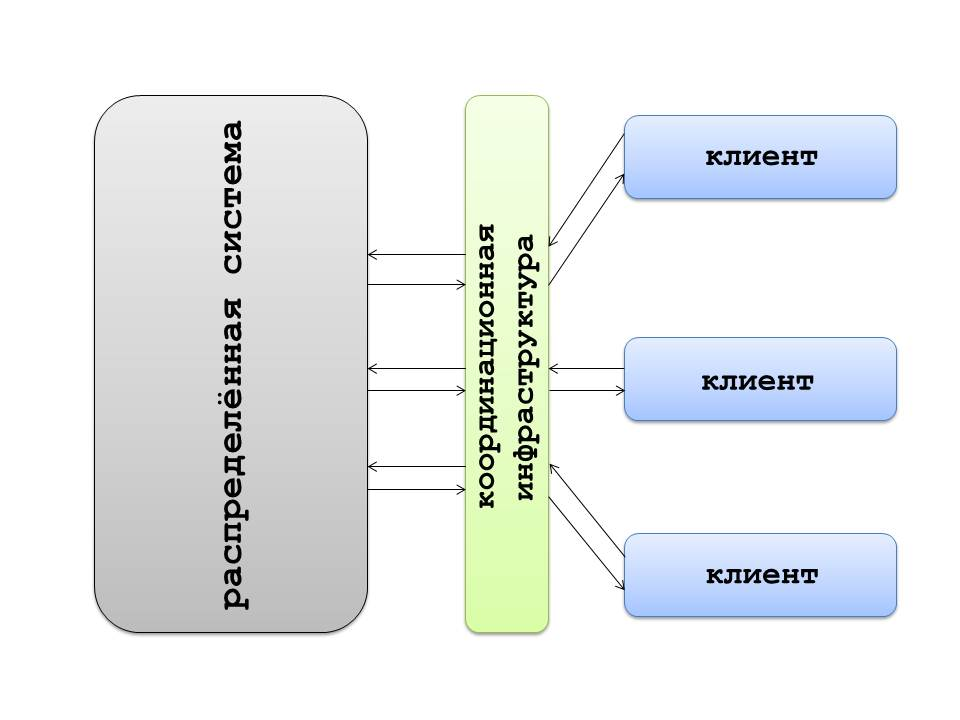
\includegraphics[width=0.7 \textwidth, height=0.5 \textwidth]{img/ClientServer}  \caption{Взаимодействие клиентов с~распределённой системой} \label{clser}
\end{figure}
Когда клиент~$p$ посылает запрос системе, этот запрос сначала обрабатывается координационной инфраструктурой и только после~этого отправляется системе. При~получении ответа от~системы координационная инфраструктура также обрабатывает полученную информацию, а затем отправляет ответ клиенту~$p$. Поэтому клиентская часть операций чтения/записи исполняется на~стороне координационной структуры, а не~на~стороне клиента.

Реализация системы~\texttt{BTS} состоит из~четырёх модулей:
\begin{itemize}
	\item модуль~\texttt{secondary\_functions} включает в~себя вспомогательные функции,
	\item модуль~\texttt{client} реализует клиентский интерфейс,
	\item модуль~\texttt{BTS\_infrastructure} реализует деятельность координационной инфраструктуры,
	\item модуль~\texttt{BTS\_server} реализует деятельность сервера~$s \in U$.
\end{itemize}
Рассмотрим реализацию компонент более подробно.


\subsection{Вспомогательные функции}\label{subsec:2}
Вспомогательные функции представлены в~модуле~\texttt{secondary\_functions}. Данный модуль включает в~себя функции сетевого взаимодействия (\texttt{get_message}, \texttt{send_message}, \texttt{connect_to_server}), а также функцию создания и записи пространства кортежей в~файл (\texttt{create_ts_file}).

Функции сетевого взаимодействия используют в~своей работе возможности модуля~\texttt{socket} из~стандартной бибилиотеки~\texttt{Python}~\autocite{socket}. Функция~\texttt{connect_to_server} принимает в~качестве входного параметра порт, к~которому необходимо подключиться (см.\,листинг~\ref{list:connect}). При~удачном подключении возвращается сокет, который можно использовать для~обмена сообщениями в~дальнейшей работе, иначе возвращается объект~\texttt{None}, сигнализирующий о~неудаче.
\begin{ListingEnv}\caption{Модуль~\texttt{secondary\_functions}, функция~\texttt{connect\_to\_server}}\label{list:connect}
\begin{lstlisting}[language=Python, numbers=left]
def connect_to_server(port):
  sock = socket(AF_INET, SOCK_STREAM)
  i = 100
  while i:
    try:
      sock.connect(('localhost', port))
    except ConnectionRefusedError:
      i -= 1
    else:
      return sock
  return None
\end{lstlisting}
\end{ListingEnv}

Функция~\texttt{send_message} используются для~отправки данных по~сети (см.\,листинг~\ref{list:send}), она имеет два входных параметра: сокет, с~помощью которого осуществляется отправка сообщения, и само сообщение, которое требуется отправить.
\begin{ListingEnv}\caption{Модуль~\texttt{secondary\_functions}, функция~\texttt{send\_message}}\label{list:send}
\begin{lstlisting}[language=Python, numbers=left]
def send_message(sock, msg):
  return sock.send(pickle.dumps(msg))
\end{lstlisting}
\end{ListingEnv}
Чтобы преобразовать сообщение к~виду, пригодному для~записи в~сокет, используется функция~\texttt{dumps} из~модуля~\texttt{pickle}~\autocite{pickle}, отвечающая за~сериализацию объектов. По~окончании операции записи в~сокет функция~\texttt{send_message} завершает свою работу и возвращает количество отправленных байт.

Функция~\texttt{get_message} используются для~получения данных из~сети (см.\,листинг~\ref{list:get}), она имеет единственный входной параметр~--- сокет, из~которого осуществляется чтение информации. Во~избежание блокировки устанавливается тайм-аут длительностью в~десять минут.
\begin{ListingEnv}\caption{Модуль~\texttt{secondary\_functions}, функция~\texttt{get\_message}}\label{list:get}
	\begin{lstlisting}[language=Python, numbers=left]
def get_message(sock):
  sock.settimeout(600)
  msg = b""
  tmp = b""
  while True:
    try:
      tmp = sock.recv(1024)
    except error:
      break
    if len(tmp) < 1024:
      break
    msg += tmp
  msg += tmp
  if len(msg) > 0:
    return pickle.loads(msg)
  return None
\end{lstlisting}
\end{ListingEnv}
Если полученное сообщение оказалось пустым, то~возвращается объект~\texttt{None}, иначе сообщение десериализуется с~помощью функции~\texttt{loads} из~модуля~\texttt{pickle} и возвращается функцией~\texttt{get_message}.

Функция~\texttt{create_ts_file} создаёт пространство кортежей и записывает его в~файл. Реализация представлена в~листинге~\ref{list:cfile}.
\begin{ListingEnv}[b]\caption{Модуль~\texttt{secondary\_functions}, функция~\texttt{create\_ts\_file}}\label{list:cfile}
	\begin{lstlisting}[language=Python, numbers=left]
def create_ts_file(file_name, init_num, amount=500, length=100):
  with open(file_name, 'w') as f:
    list_of_tuples = list()
    for i in range(init_num * amount, (init_num + 1) * amount):
      list_of_tuples.append(tuple(j for j in range(i, i+length)))
    json.dump(list_of_tuples, f)
	\end{lstlisting}
\end{ListingEnv}
Данная функция используется для~того, чтобы в~дальнейшем каждый сервер системы при~запуске смог прочитать информацию из~созданного при~помощи~\texttt{create_ts_file} файла и сконструировать локальную реплику пространства кортежей. Имя файла, объём создаваемого пространства, а также длина и значения полей входящих в~него кортежей регулируются входными параметрами функции. Для~преобразования созданного пространства кортежей в~удобный формат и дальнейшей записи его в~файл используется функция~\texttt{dump} из~модуля~\texttt{json}~\autocite{json}.


\subsection{Клиентский интерфейс}\label{subsec:3}
Интерфейс пользователя для~взаимодействия с~\texttt{BTS} реализован с~помощью класса~\texttt{Client} из~модуля~\texttt{client} (полный программный код представлен в~\autocite{mybts}). Для~того, чтобы начать работу, следует создать объект класса~\texttt{Client}, передав конструктору в~качестве входного параметра значение порта, который координационная инфраструктура использует для~обмена сообщениями с~клиентами.

Ввиду возможности возникновения ошибок для~контроля исполняемых операций используется модуль~\texttt{logging}~\autocite{logging} из~стандартной библиотеки языка~\texttt{Python}, отвечающий за~логирование. Создание и настройка конфигурации лога происходит в~конструкторе класса~\texttt{Client} следующим образом:
\begin{lstlisting}[language=Python]
  logging.basicConfig(filename='client_log.txt', level=logging.INFO, format="%(asctime)s - %(message)s")
\end{lstlisting}
При~помощи функции~\texttt{basicConfig} устанавливается имя файла для~записи лога, уровень логирования и формат выводимых сообщений.

Для~исполнения операций чтения/записи необходимо вызвать соответствующую функцию: \texttt{out_op($t$)}, \texttt{rd_op($\bar t$)} или \texttt{in_op($\bar t$)} (см.\,листинг~\ref{list:clops}).
\begin{ListingEnv}[H]\caption{Модуля~\texttt{client}, методы~\texttt{out\_op}, \texttt{rd\_op}, \texttt{in\_op}}\label{list:clops}
	\begin{lstlisting}[language=Python, numbers=left]
def out_op(self, tup):
  self.__op('out', tup)
  logging.info('OUT: ' + str(tup))

def rd_op(self, temp):
  resp = self.__op('rd', temp)
  logging.info('RD: ' + str(resp))
  return resp

def in_op(self, temp):
  resp = self.__op('in', temp)
  logging.info('IN: ' + str(resp))
  return resp
\end{lstlisting}
\end{ListingEnv}
Заметим, что операция записи~\texttt{out_op} в~качестве входного параметра принимает кортеж, а операции чтения~\texttt{rd_op}~и~\texttt{in_op}~--- шаблон кортежа. Каждая из~этих операций исполняется путём вызова приватного метода~\texttt{\_\_op} (см.\,листинг~\ref{list:clop}).
\begin{ListingEnv}\caption{Модуль~\texttt{client}, приватный метод~\texttt{op}}\label{list:clop}
	\begin{lstlisting}[language=Python, numbers=left]
def __op(self, op_type, tup=None):
  sock = connect_to_server(self.port)
  if sock is not None:
    if op_type == 'out':
      req = {'op': op_type, 'tup': tup}
    elif op_type in ['rd', 'in']:
      req = {'op': op_type, 'temp': tup}
    elif op_type == 'stop':
      req = {'op': op_type}
    send_message(sock, req)
    if op_type in ['rd', 'in', 'stop']:
      resp = get_message(sock)
      sock.close()
      if resp is None:
        return resp
      return resp['resp']
    else:
      sock.close()
  else:
    logging.info(str(op_type) + ': cannot connect to server')
    return None
	\end{lstlisting}
\end{ListingEnv}
Внутри~данного метода формируется запрос в~виде словаря~\texttt{\{'op': код операции, 'tup': кортеж\}} или \texttt{\{'op': код операции, 'temp': шаблон кортежа\}}, содержание которого соответствует семантике исполняемой операции. Сформированный запрос отправляется координационной инфраструктуре. Для~завершения операции записи ответ системы не~требуется, а операции чтения ожидают, когда инфраструктура вернёт запрошенное значение.

Для~корректного завершения работы системы в~классе~\texttt{Client} реализована функция~\texttt{stop_op} (см.\,листинг~\ref{list:clstop}), при~исполнении которой инфраструктуре отправляется запрос о~прекращении работы и ожидается ответ об~успешном результате операции.
\begin{ListingEnv}\caption{Модуль~\texttt{client}, метод~\texttt{stop_op}}\label{list:clstop}
	\begin{lstlisting}[language=Python, numbers=left]
def stop_op(self):
  resp = self.__op('stop')
  logging.info('STOP: ' + str(resp))
  return resp
	\end{lstlisting}
\end{ListingEnv}
По~смыслу данная функция не~должна являться частью клиентского интерфейса, она была включена в~класс~\texttt{Client} для~удобства.


\subsection{Координационная инфраструктура}\label{subsec:4}
Координационная инфраструктура системы~\texttt{BTS} реализована в~модуле~\texttt{BTS_infrastructure} с~помощью класса~\texttt{BTS_infrastructure} (полный программный код представлен в~\autocite{mybts}). Она представляет собой многопоточное приложение, которое обрабатывает запросы клиента и взаимодействует с~серверами системы~\texttt{BTS}.

Для~того, чтобы настроить работу координационной системы, необходимо создать объект класса~\texttt{BTS_infrastructure} и передать в~его конструктор следующие параметры:
\begin{itemize}
	\item порт, который будет прослушивать инфраструктура и на~который будут поступать клиентские запросы,
	\item список портов, каждый из~которых будет прослушивать определённый сервер системы~\texttt{BTS},
	\item количество неисправных серверов (предателей), которые будут порождать конфликты в~системе,
	\item размер кворума записи,
	\item размер кворума чтения,
	\item имя файла, в~котором хранится множество кортежей для~корректных серверов,
	\item имя файла, в~котором хранится множество кортежей для~неисправных серверов.
\end{itemize}
В~теле конструктора значения входных параметров присваиваются соответствующим свойствам класса, устанавливается значение флага~\texttt{THREAD_POOL_ON} (данный флаг используется при~обработке клиентских запросов), значение свойства~\texttt{AMOUNT_OF_CLIENTS} устанавливается в~нуль (данное свойство является счётчиком поступивших клиентских запросов), множество серверов~$U$ разбивается на~кворумы записи~$Q_w$ и чтения~$Q_r$, а также настраивается конфигурация лога.

После создания объекта класса для~запуска работы координационной инфраструктуры необходимо вызвать метод~\texttt{run} (см.\,листинг~\ref{list:infrun1}).
\begin{ListingEnv}\caption{Модуль~\texttt{BTS\_infrastructure}, метод~\texttt{run}}\label{list:infrun1}
\begin{lstlisting}[language=Python, numbers=left]
def run(self):
  if self.AMOUNT_OF_ENEMIES >= self.AMOUNT_OF_SERVERS:
    return False
  self.start_servers(0, self.AMOUNT_OF_ENEMIES, self.WRONG_TS_FILE)
  self.start_servers(self.AMOUNT_OF_ENEMIES, self.AMOUNT_OF_SERVERS, self.TS_FILE)
  .........
	\end{lstlisting}
\end{ListingEnv}
Если изначально количество неисправных серверов было указано неверно, то~есть не~меньше количества всех имеющихся серверов, то возвращается значение~\texttt{False}. Иначе работа функции продолжается: происходит запуск корректных и неисправных серверов с~помощью метода~\texttt{start_servers} (см.\,листинг~\ref{list:infstartserv}).
\begin{ListingEnv}\caption{Модуль~\texttt{BTS\_infrastructure}, метод~\texttt{start\_servers}}\label{list:infstartserv}
	\begin{lstlisting}[language=Python, numbers=left]
def start_servers(self, ind1, ind2, file):
  for i in range(ind1, ind2):
    try:
      Popen('python BTS_server.py '+str(i)+' '+str(self.U[i])+' '+str(file)+' '+''.join(str(j)+' ' for j in self.U), stdout=PIPE, stderr=PIPE, shell=True)
    except CalledProcessError:
      logging.info('START_SERVERS: cannot start server ' + str(self.U[i]))
    else:
      logging.info('START_SERVERS: start server '+str(self.U[i]))
	\end{lstlisting}
\end{ListingEnv}
Метод~\texttt{start_servers} имеет три входных параметра:
\begin{itemize}
	\item два индекса, определяющие диапазон значений в~списке портов~\texttt{self.U}, которые будут прослушивать запускаемые серверы,
	\item имя файла, которое будет подано выбранным серверам на~вход.
\end{itemize}
Программная реализация сервера системы~\texttt{BTS} представлена в~модуле~\texttt{BTS_server}, который будет рассмотрен позже в~разделе~\ref{subsec:5}, данный скрипт~\texttt{BTS_server.py} запускается с~определёнными параметрами в~новом процессе при~помощи конструктора класса~\texttt{Popen} из~модуля~\texttt{subprocess}~\autocite{subprocess} стандартной библиотеки~\texttt{Python}. В~скрипт передаются следующие аргументы:
\begin{itemize}
	\item идентификатор сервера,
	\item порт, который будет прослушивать сервер,
	\item имя файла с~хранящимся в~нём пространством кортежей,
	\item список портов всех серверов.
\end{itemize}

Вернёмся к~методу~\texttt{run}. После~запуска серверов создаётся и настраивается сокет, с~помощью которого далее будет происходить коммуникация с~клиентскими процессами (см.\,листинг~\ref{list:infrun2}). Клиентские запросы будут обрабатываться при~помощи пула потоков~\texttt{ThreadPoolExecutor} из~модуля~\texttt{concurrent.futures}~\autocite{concurrent} стандартной библиотеки~\texttt{Python}, принимающего в~качестве аргумента количество потоков, используемых в~работе.
\begin{ListingEnv}\caption{Модуль~\texttt{BTS\_infrastructure}, метод~\texttt{run} (продолжение)}\label{list:infrun2}
	\begin{lstlisting}[language=Python, numbers=left]
  .........
  s = socket(AF_INET, SOCK_STREAM)
  s.bind(('', self.INFRASTRUCTURE_PORT))
  s.listen(1)
  with ThreadPoolExecutor(10) as pool:
    while self.THREAD_POOL_ON:
      try:
        s.settimeout(30)
        client_s, client_addr = s.accept()
        self.AMOUNT_OF_CLIENTS += 1
      except error:
        pass
      else:
        pool.submit(self.worker,client_s,self.AMOUNT_OF_CLIENTS)
  s.close()  
  logging.info('RUN: stop working')
  return True
	\end{lstlisting}
\end{ListingEnv}
Пока флаг~\texttt{THREAD_POOL_ON} равен~\texttt{True}, исполняется следующая последовательность инструкций: ожидается подключение клиента к~порту, создаётся соответствующий клиентский сокет, количество полученных клиентских запросов увеличивается на~единицу. При~удачном завершении описанных инструкций задача с~помощью метода~\texttt{submit} добавляется в~очередь для~исполнения пулом потоков. Метод~\texttt{submit} принимаюет в~качестве входных параметров имя функции~(\texttt{worker}), которую необходимо исполнить в~одном из~потоков пула, и значения аргументов (клиентский сокет и \texttt{AMOUNT_OF_CLIENTS}), с~которыми эта функция будет запущена.

Флаг~\texttt{THREAD_POOL_ON} может изменить своё значение только при~получении запроса о~прекращении работы от~клиента. Если это произошло, то~новые задачи перестают добавляться в~очередь пула потоков, ожидается завершение всех исполняющихся или ожидающих в~очереди задач.

На~этом работа метода~\texttt{run} прекращается, возвращается значение~\texttt{True}, свидетельствующее об~успешном завершении работы координационной инфраструктуры.

Заметим, что метод~\texttt{run} является блокирующим, то~есть после~запуска инфраструктуры и вплоть до~её завершения продолжить дальнейшую работу будет невозможно.

Рассмотрим метод~\texttt{worker} (см.\,листинг~\ref{list:infworker}) более подробно. Он выполняет функцию получения и обработки запроса клиента, принимает в~качестве входных параметром клиентский сокет и идентификатор клиентского процесса.
\begin{ListingEnv}\caption{Модуль~\texttt{BTS\_infrastructure}, метод~\texttt{worker}}\label{list:infworker}
	\begin{lstlisting}[language=Python, numbers=left]
def worker(self, client, pid):
  req = get_message(client)
  if req is not None:
    try:
      if req['op'] == 'out':
        self.out(req['tup'])
      elif req['op'] == 'rd':
        send_message(client,{'resp': self.rdp(req['temp'])})
      elif req['op'] == 'in':
        send_message(client,{'resp': self.inp(pid,req['temp'])})
      elif req['op'] == 'stop':
        self.THREAD_POOL_ON = False
        self.stop_servers()
        send_message(client, {'resp': 'ok'})
      else:
        logging.info('WORKER: wrong request ' + str(req))
    except KeyError:
      logging.info('WORKER: wrong request ' + str(req))
    client.close()
	\end{lstlisting}
\end{ListingEnv}
Вспомним, что в~функцию~\texttt{submit} (добавление задачи в~очередь пула потоков) в~качестве второго аргумента функции~\texttt{worker} передаётся значение свойства~\texttt{AMOUNT_OF_CLIENTS}. Данное свойство используется для~подсчёта клиентских запросов, будем пологать, что каждый клиентский запрос был послан уникальным клиентом (согласно~системной модели~\texttt{BTS} множество клиентских процессов бесконечно), тогда в~качестве идентификатора клиентского процесса можно использовать номер запроса, что и осуществляется при~помощи свойства~\texttt{AMOUNT_OF_CLIENTS}.

Работу метода~\texttt{worker} можно разделить на~два этапа: получение сообщения от~клиента и обработка полученного запроса. Для~того, чтобы получить сообщение с~запросом от~клиента, используется функция~\texttt{get_message} из~описанного в~разделе~\ref{subsec:2} модуля~\texttt{secondary\_functions}. После~получения запроса определяется код операции, которую необходимо исполнить, вызывается соответствующая функция и при~необходимости отправляется ответ клиенту.

При~получении запросов на~исполнение операций~$out$, $rd$ или~$in$ вызываются методы~\texttt{out}, \texttt{rdp} или~\texttt{inp}, которые будут рассмотрены позже в~разделах~\ref{subsec:6}, \ref{subsec:7} и~\ref{subsec:8} соответственно.

При~получении запроса на~исполнение операции~$stop$ флаг~\texttt{THREAD_POOL_ON} устанавливается в~значение~\texttt{False}, после~чего прекращается обработка клиентских запросов, вызывается метод~\texttt{stop_servers} (см.\,листинг \ref{list:infstopserv}), при~исполнении которого всем запущенным серверам посылается запрос о~завершении работы и ожидается ответ об~удачном исходе данной операции.
\begin{ListingEnv}\caption{Модуль~\texttt{BTS\_infrastructure}, метод~\texttt{stop\_servers}}\label{list:infstopserv}
	\begin{lstlisting}[language=Python, numbers=left]
def stop_servers(self):
  for i in self.U:
    s = connect_to_server(i)
    if s is not None:
      send_message(s, {'op': 'stop'})
      resp = get_message(s)
      s.close()
      if resp['resp'] != 'ok':
        logging.info('STOP_SERVERS: cannot stop server '+str(i))
      else:
        logging.info('STOP_SERVERS: stop server '+str(i))
    else:
      logging.info('STOP_SERVERS: cannot stop server '+str(i))
	\end{lstlisting}
\end{ListingEnv}


\subsection{Серверная составляющая системы}\label{subsec:5}
Серверная составляющая системы~\texttt{BTS} реализована в~модуле~\texttt{BTS_server} (полный программный код представлен в~\autocite{mybts}), он представляет собой скрипт, запуск которого приводит в~исполнение сервер системы. Как уже было отмечено в~разделе~\ref{subsec:4}, скрипт запускается со~следующими аргументами:
\begin{itemize}
	\item идентификатор сервера,
	\item порт, который будет прослушивать сервер,
	\item имя файла с~хранящимся в~нём пространством кортежей,
	\item список портов всех серверов.
\end{itemize}
Для~обработки аргументов используется библиотека~\texttt{argparse}~\autocite{argparse}. Она предоставляет возможности анализа аргументов командной строки, конвертирования стркоовых аргументов в~другие объекты программы и вывода информационных подсказок.

Для~мониторинга работы сервера настраивается логирование.

При~запуске сервер считывает из~полученного файла кортежи и создаёт локальную копию пространства кортежей при~помощи функции~\texttt{read_from_ts_file} (см.\,листинг~\ref{list:servreadts}).
\begin{ListingEnv}\caption{Модуль~\texttt{BTS\_server}, функция~\texttt{read\_from\_ts\_file}}\label{list:servreadts}
	\begin{lstlisting}[language=Python, numbers=left]
def read_from_ts_file(file_name):
  global TS
  with open(file_name, 'r') as f:
    data = json.load(f)
    for i in data:
      TS.add(tuple(i))
	\end{lstlisting}
\end{ListingEnv}
На~сервере кортежи хранятся в~контейнере~\texttt{set} (переменная~\texttt{TS}), что позволяет исключить наличие идентичных кортежей и сделать проверку на~вхождение быстрой, поскольку~\texttt{set} в~качестве базовой структуры данных использует хэш-таблицу~\autocite{Gorelick}.

Далее, как и в~случае с~координационной инфраструктурой, создаётся сокет, через~который будет осуществляться коммуникация с~инфраструктурой, запускается пул потоков~\autocite{threadpool} и начинается обработка входящих запросов.

Обработка входящих запросов осуществляется при~помощи функции~\texttt{worker}, её программная реализация практически идентична одноимённой функции из~модуля~\texttt{BTS\_infrastructure} и не~нуждается в~представлении. В~теле данной функции сначала происходит считывание сообщения, полученного от~инфраструктуры, далее по~содержимому полученного сообщения определяется тип комнады и вызывается соответствующая одноимённая функция. Полный перечень возможных команд приведён ниже:
\begin{itemize}
	\item \texttt{out}~--- команда операции записи~$out$,
	\item \texttt{rd}~--- команда операции недеструктивного чтения~$rd$,
	\item \texttt{in}~--- команда операции деструктивного чтения~$in$,
	\item \texttt{enter}~--- команда входа в~критическую секцию,
	\item \texttt{exit}~--- команда выхода из~критической секции,
	\item \texttt{accept1}~--- команда первого этапа утверждения удаляемого кортежа,
	\item \texttt{accept2}~--- команда второго этапа утверждения удаляемого кортежа,
	\item \texttt{stop}~--- команда о~прекращения работы сервера.
\end{itemize}
Первые три команды связаны с~операциями манипулирования кортежами, следующие четыре команды~--- с~реализацией операции~$in$ (они будут рассмотрены позже в~разделе~\ref{subsec:8}). Последняя команда~\texttt{stop} устанавливает флаг~\texttt{THREAD_POOL_ON} в~значение~\texttt{False}, что приводит к~прекращению работы пула потоков, а затем~--- к~завершению работы сервера.


\subsection{Операция записи out}\label{subsec:6}
Операция~$out(t)$ добавляет кортеж~$t$ в~пространство кортежей. На~стороне инфраструктуры эта операция реализуется с~помощью метода~\texttt{out(self, t)}, программный код которого приведён в~листинге~\ref{list:infout}.
\begin{ListingEnv}\caption{Модуль~\texttt{BTS\_infrastructure}, метод~\texttt{out}}\label{list:infout}
	\begin{lstlisting}[language=Python, numbers=left]
def out(self, t):
  for i in self.QW:
    sock = connect_to_server(i)
    if sock is not None:
      send_message(sock, {'op': 'out', 'tup': t})
      logging.info('OUT: send '+str(t)+' to server '+str(i))
      sock.close()
    else:
      logging.info('OUT: cannot connect to server ' + str(i))
  logging.info('OUT: recorded ' + str(t))
	\end{lstlisting}
\end{ListingEnv}
Для~того, чтобы добавить кортеж~$t$ в~пространство, производится подключение к~серверам системы, состоящим в~кворуме записи, и в~случае удачного подключения отправляется запрос~\texttt{\{'op': 'out', 'tup': t\}} на~добавление кортежа.

Заметим, что при~вызове данной функции ждать ответа от~серверов нет необходимости. Будем считать, что операция завершится в~тот момент, когда все корректные серверы из~кворума записи получат кортеж~$t$.

На~стороне сервера операция~$out(t)$ реализуется с~помощью функции~\texttt{out(t)} (см.\,листинг~\ref{list:servout}).
\begin{ListingEnv}\caption{Модуль~\texttt{BTS\_server}, функция~\texttt{out}}\label{list:servout}
	\begin{lstlisting}[language=Python, numbers=left]
def out(t):
  global TS, RS
  if t not in RS:
    TS.add(t)
    logging.info('OUT: add ' + str(t) + ' to TS')
  try:
    RS.remove(t)
  except KeyError:
    pass
  else:
    logging.info('OUT: remove ' + str(t) + ' from RS')
	\end{lstlisting}
\end{ListingEnv}
При~получении запроса на~добавление кортеж~$t$ добавляется в~пространство кортежей только в~том случае, если этот кортеж ранее не~был из~него удалён (то~есть его нет во~множестве~\texttt{RS}). Это необходимо для~того, чтобы один и тот~же кортеж не~был удалён дважды.


\subsection{Операция чтения rd}\label{subsec:7}
Операция недеструктивного чтения~$rd(\bar t)$ в~качестве входного параментра принимает шаблон кортежа~$\bar t$ и возвращает копию кортежа, соответствующего шаблону, не~извлекая его из~пространства. Реализация этой операции на~стороне инфраструктуры представлена в~виде метода~\texttt{rdp(self, temp, ts=None)} (полный программный код приведён в~\autocite{mybts}), имеющего два параметра: шаблон кортежа и объект~\texttt{ts} (по~умолчанию равный~\texttt{None}), значение которого будет объяснено позже. При~получении запроса на~исполнение операции~$rd$ функция~\texttt{rdp} вызывается с~единственным первым параметром.

\begin{ListingEnv}\caption{Модуль~\texttt{BTS\_infrastructure}, метод~\texttt{rdp}}\label{list:infrdp1}
	\begin{lstlisting}[language=Python, numbers=left]
def rdp(self, temp, ts=None):
  if ts is None:
    ts = {i: [None, None] for i in self.QR}  #port: (socket, set)
    for i in self.QR:
      ts[i][0] = connect_to_server(i)
      if ts[i][0] is not None:
        send_message(ts[i][0], {'op': 'rd', 'temp': temp})
        logging.info('RDP: send '+str(temp)+' to server '+str(i))
      else:
        ts.pop(i)
    for i in ts.keys():
      msg = get_message(ts[i][0])
      ts[i][0].close()
      if msg is not None:
        ts[i][1] = msg['ts']
      else:
        ts[i][1] = None
      logging.info('RDP: receive ' + str(ts[i][1]) + ' from server ' + str(i))
  .........
	\end{lstlisting}
\end{ListingEnv}

Суть работы функции заключается в~следующем. Каждому серверу из~кворума чтения посылается запрос на~исполнение операции~$rd(\bar t)$ (см.\,листинг~\ref{list:infrdp1}). Ответы от~серверов кворума приходят в~виде множества подходящих под~шаблон~$\bar t$ кортежей и записываются в~словарь~\texttt{ts}, имеющий структуру: \texttt{port: (socket, set)}, где~\texttt{port}~--- порт, который прослушивает конкретный сервер, \texttt{socket}~--- сокет, с~помощью которого происходит коммуникация, \texttt{set}~--- множество подходящих кортежей, хранящихся на~данном сервере. Заметим, что словарь~\texttt{ts} может передаваться в~функцию уже в~готовом виде, этот факт используется в~реализации операции~$in(\bar t)$, которая будет рассмотрена в~разделе~\ref{subsec:8}.

Из~всех полученных кортежей выбирается один общий кортеж~$t$, который располагается как~минимум на~$f + 1$ сервере (см.\,листинг~\ref{list:infrdp2}).
\begin{ListingEnv}\caption{Модуль~\texttt{BTS\_infrastructure}, метод~\texttt{rdp} (продолжение)}\label{list:infrdp2}
	\begin{lstlisting}[language=Python, numbers=left]
  .........
  t = None
  for i in combinations(ts.keys(), self.AMOUNT_OF_ENEMIES + 1):
    ts_intersection = ts[i[0]][1]
    for j in i:
      if ts[j][1] is None:
        ts_intersection = None
        break
      ts_intersection = ts_intersection.intersection(ts[j][1])
      if len(ts_intersection) == 0:
        break
    if ts_intersection is not None:
      if len(ts_intersection) > 0:
        t = ts_intersection.pop()
        break
  logging.info('RDP: selected ' + str(t))
  return t
	\end{lstlisting}
\end{ListingEnv}
Чтобы найти кортеж~$t$, необходимо подобрать такую комбинацию из~$f + 1$ сервера, пересечение множеств подходящих кортежей которых будет непусто. Для~этого рассматриваются всевозможные сочетания из~$f + 1$ сервера при~помощи функции~\texttt{combinations} из~модуля~\texttt{itertools}~\autocite{itertools}. Для~нахождения пересечений множеств подходящих кортежей используются методы класса~\texttt{set}~\autocite{set}. После~нахождения кортежа~$t$ он возвращается в~качестве выходного параметра. Если подходящего кортежа не~нашлось, то возвращается объект~\texttt{None}, свидетельствующий о~том, что операция чтения не~увенчалась успехом.

Рассмотрим реализацию функции недеструктивного чтения~\texttt{rdp(sock, temp)} на~стороне сервера (см.\,листинг~\ref{list:servrdp}). Функция принимает два входных параметра: сокет и шаблон кортежа.
\begin{ListingEnv}\caption{Модуль~\texttt{BTS\_server}, функция~\texttt{rdp}}\label{list:servrdp}
	\begin{lstlisting}[language=Python, numbers=left]
def rdp(sock, temp):
  global TS
  temp_set = set()
  for t in TS:
    if match(temp, t):
      temp_set.add(t) 
  logging.info('RDP: temp '+str(temp)+', set '+str(temp_set))
  if sock is not None:
    send_message(sock, {'ts': temp_set})
  else:
    return temp_set
	\end{lstlisting}
\end{ListingEnv}
Для~того, чтобы найти подходящие под~шаблон кортежи, производится один проход по~локальной копии пространства кортежей~\texttt{TS}, каждый кортеж которого проверяется на~пригодность функцией~\texttt{match}. Если функция~\texttt{match} вернула значение~\texttt{True}, то~кортеж добавляется во~множество подходящих кортежей~\texttt{temp_set}, иначе игнорируется.

Функция~\texttt{match(temp, t)} проверяет, соответствует~ли кортеж~\texttt{t} шаблону~\texttt{temp}: сначала происходит сравнение длин шаблона и кортежа, в~случае их совпадения сравниваются определённые в~шаблоне поля с~соответствующими полями проверяемого кортежа. Если длины кортежей оказались разными или какое-то определённое поле шаблона не~совпало с~соответствующим полем кортежа, то возвращается значение~\texttt{False}, говорящее о~том, что кортеж не~подходит под~шаблон. Иначе возвращается значение~\texttt{True}. Программная реализация данной функции представлена в~\autocite{mybts}.

Если переданный в~функцию~\texttt{rdp} сокет оказался не~равен значению~\texttt{None}, то полученное множество~\texttt{temp_set} отправляется инфраструктуре в~качестве ответа. Иначе оно возвращается в~качестве выходного параметра. Такая архитектура необходима для~реализации операции~$in(\bar t)$, которая будет рассмотрена в~следующем разделе.


\subsection{Операция чтения in}\label{subsec:8}
Операция деструктивного чтения~$in$ имеет более сложную реализацию, поскольку один кортеж не~может быть удалён из~пространства двумя различными вызовами~$in$. Этот факт подразумевает использование критических секций для~процессов, пытающихся удалить один и тот~же кортеж, что, во-первых, обеспечит невозможность удаления кортежа двумя процессами одновременно, во-вторых, позволит всем процессам получить доступ к~ресурсу в~некоторое время.

Помимо~критических секций необходимо использовать алгоритм достижения консенсуса~\autocite{paxos}, чтобы в~результате исполнения операции~$in$ из~пространства был удалён правильный кортеж. Ярким представителем таких алгоритмов является алгоритм~Paxos, предложенный Лесли Лампортом~\autocite{Lamport}.

Paxos~--- это алгоритм решения задачи консенсуса в~сети ненадёжных вычислителей. Компоненты распределённой системы можно разделить на~три группы~\autocite{paxos}:
\begin{itemize}
	\item Заявитель (Proposer)~--- выдвигает <<предложения>> (какие-то значения), которые либо принимаются, либо отвергаются в~результате работы алгоритма.
	\item Акцептор (Acceptor)~--- принимает или отвергает <<предложение>> Заявителя, согласует своё решение с~остальными Акцепторами, уведомляет о~своём решении Узнающих. Если Акцепторами было принято какое-либо значение, предложенное Заявителем, то оно называется утверждённым.
	\item Ученик (Learner)~--- запоминает решение Акцепторов, принятое в~результате работы алгоритма консенсуса.
\end{itemize}

Компоненты распределённой системы могут принадлежать сразу нескольким группам, описанным выше, и вести себя и как Заявитель, и как Акцептор, и как Ученик. Такое распределение ролей в~системе гарантирует следующее~\autocite{Lamport}:
\begin{itemize}
	\item Только предложенное Заявителем значение может быть утверждено Акцепторами.
	\item Акцепторами утверждается только одно значение из~всех предложенных Заявителями значений (возможно, противоречивых).
	\item Ученик не~сможет узнать об~утверждении какого-либо значения вплоть до~того момента, пока оно действительно не~будет утверждено.
\end{itemize}

Распределим роли среди компонент системы~\texttt{BTS} следующим образом:
\begin{itemize}
	\item Множество Заявителей состоит только из~координационной инфраструктуры. Такой набор гарантирует наличие корректного Заявителя.
	\item Множество Акцепторов составляют все серверы системы.
	\item Множество Учеников включает в~себя все серверы системы и инфраструктуру.
\end{itemize}

Рассмотрим реализацию операции~$in(\bar t)$ на~стороне инфраструктуры, представленную методом~\texttt{inp(self, pid, temp)} (см.\,листинг~\ref{list:infinp}). 
\begin{ListingEnv}\caption{Модуль~\texttt{BTS\_infrastructure}, метод~\texttt{inp}}\label{list:infinp}
	\begin{lstlisting}[language=Python, numbers=left]
def inp(self, pid, temp):
  while True:
    t, ts = self.enter_r(pid, temp)
    logging.info('INP: enter with pid ' + str(pid) + ', temp ' + str(temp) + ', t: ' + str(t))
    if t is None:
      self.exit_r(pid, temp)
      logging.info('INP: exit from cs with pid ' + str(pid))
      return None
    d = self.paxos(pid, temp, t, ts)   
    if d == t:
      break
  logging.info('INP: pid ' + str(pid) + ' deleted ' + str(t))
  return t
	\end{lstlisting}
\end{ListingEnv}
Функция~\texttt{inp} принимает два параметра: идентификатор клиентского процесса и шаблон кортежа. В~первую очередь инфраструктура пытается войти в~критическую секцию системы для~удаления подходящего под~шаблон~\texttt{temp} кортежа.

Функция входа в~критическую секцию~\texttt{enter_r(self, pid, temp)} совмещена с~операцией недеструктивного чтения~$rd(\bar t)$. Это необходимо для~того, чтобы уменьшить количество обращений к~системе и, как~следствие, ускорить исполнение операции~$in$. Сначала всем серверам системы отправляется запроса на~вход в~критическую секцию, от~каждого сервера ожидается ответ. В~качестве ответа возврщается сообщение вида~\texttt{\{'resp': 'go', 'ts': ts\}}, где~\texttt{ts}~--- это множество кортежей, соответствующих шаблону~\texttt{temp}. Далее с~помощью метода~\texttt{rdp}, описанного в~предыдущем разделе, из~полученных множеств~\texttt{ts} выбирается конкретный кортеж для~удаления. Программная реализация метода~\texttt{enter_r} представлена в~\autocite{mybts}.
		
Таким образом, по~окончании выполнения функции~\texttt{enter_r} все серверы уже разрешили войти в~свои критические секции, а инфраструктурой уже был выбран кортеж~$t$ для~удаления.

Если не~удалось выбрать подходящий кортеж~$t$, то вызывается метод~\texttt{exit_r(self, pid, temp)}, который посылает серверам запрос на~выход из~критической секции без~ожидания ответа. После~этого метод~\texttt{inp} возвращает значение~\texttt{None}, свидетельствующее о~том, что подходящего для~удаления кортежа нет в~пространстве.

Если же выбрать кортеж~$t$ всё-таки получилось, то необходимо выяснить, можно~ли удалить этот кортеж из~пространства. Для~этого вызывается метод~\texttt{paxos(self, pid, temp, t, ts)}, в~ходе исполнения которого серверам системы отправляется предложение об~удаление кортежа~$t$, после~чего от~каждого сервера приходит ответ о~принятом решении. На~основе ответов серверов средствами модуля~\texttt{collections}~\autocite{collections} выбирается самый популярный ответ (см.\,листинг~\ref{list:infpaxos}). Если данное значение утвердил хотя~бы~$f + 1$ сервер, оно возвращается в~качетсве выходного параметра, иначе возвращается~\texttt{None}.
\begin{ListingEnv}\caption{Модуль~\texttt{BTS\_infrastructure}, метод~\texttt{paxos}}\label{list:infpaxos}
	\begin{lstlisting}[language=Python, numbers=left]
def paxos(self, pid, temp, t, ts):
  .........
  c = Counter(tup_list)
  mc = c.most_common(1)[0]
  if mc[1] > self.AMOUNT_OF_ENEMIES:
    return mc[0]
  return None
	\end{lstlisting}
\end{ListingEnv}
Заметим, что в~случае наличия~$f$ и менее неисправных серверов в~качестве ответа от~сервера может прийти либо кортеж~$t$ (значит он уже был удалён из~пространства), либо объект~\texttt{None} (удаления не~произошло), поскольку ни~один сервер не~является Заявителем. Таким образом, метод~\texttt{paxos} симулирует деятельность инфраструктуры как Заявителя и Ученика.

Данный результат иллюстрирует благоприятный и промежуточный исходы задачи византийских генералов. При~благоприятном исходе из~пространства кортежей удаляется кортеж, предложенный клиентом, то~есть приказ главнокомандующего (клиента) был получен и изучен всеми генералами (серверами), после~чего они единогласно приняли решение следовать приказу. При~промежуточном исходе кортеж не~удаляется, возвращается~\texttt{None}, при~этом сохраняется целостность пространства кортежей, поскольку на~всех корректных серверах удаления не~произошло. Иными словами, генералами (серверами) было принято единогласное решение не~доверять приказу главнокомандующего (клиента) и отступить (не~производить удаление), сохранив при~этом армию (целостность пространства кортежей).

На~момент выхода из~метода~\texttt{paxos} все серверы уже сделали выбор, какой именно кортеж удалять. Если функция~\texttt{paxos} вернула значение, равное~$t$, то операция~$in$ считается успешно завершённой и возвращается кортеж~$t$. В~противном случае необходимо произвести ту~же последовательность действий, начиная со~входа в~критическую секцию. Данный процесс продолжается до~того момента, пока серверами не~будет одобрено предложенное инфраструктурой значение или пока в~пространстве не~окажется подходящих для~удаления кортежей.

Заметим, что выход из~критической секции происходит только в~случае неудачного исхода операции удаления, а в~остальных случаях этого не~происходит, поскольку выход из~критической секции на~каждом сервере осуществляется локально, и при~следующей попытке инфраструктуры войти в~критическую секцию не~возникает проблем. Такая реализация необходима для~избежания блокировок.

Теперь рассмотрим реализацию операции~$in$ на~стороне сервера. Исполнение операции~$in$ на~стороне инфраструктуры начинается с~попытки входа в~критическую секцию, рассмотрим, что происходит на~сервере в~этот момент. При~получении запроса на~вход в~критическую секцию вызывается функция~\texttt{enter_r(sock, pid, temp)} (программная реализация приведена в~\autocite{mybts}), выполняющая две операции: добавление запроса в~очередь и конструирование множества кортежей, подходящих под~шаблон~\texttt{temp}.

Когда инфраструктура запрашивает доступ к~критической секции, происходит захват ресурса~--- типа шаблона кортежа. Тип шаблона кортежа~--- это кортеж, поля которого равны значениям типов соответствующих полей шаблона. Если тип шаблона уже захвачен другим вызовом~\texttt{enter_r}, то запрос добавляется в~очередь, соответствующую данному ресурсу. Иначе происходит захват типа шаблона и исполняются инструкции, отвечающие за~конструирование множества кортежей, соответствующих шаблону, с~помощью функции~\texttt{rdp}.

Далее инфраструктура посылает серверам запрос на~удаление конкретного кортежа. При~получении данного запроса вызывается функция~\texttt{inp(sock, pid, temp, tup)} с~аргументами: сокет, идентификатор клиентского процесса, шаблон кортежа и кортеж, предложенный для~удаления (см.\,листинг~\ref{list:servinp}).
\begin{ListingEnv}\caption{Модуль~\texttt{BTS\_server}, функция~\texttt{inp}}\label{list:servinp}
	\begin{lstlisting}[language=Python, numbers=left]
def inp(sock, pid, temp, tup):
  global TS, RS, QR, TYPES
  logging.info('INP ' + str(pid) + ': propose ' + str(tup))
  if QR[TYPES[temp]][0][1] == pid:
    d = paxos(sock, temp, tup)
    if d is not None:
      if d not in TS:
        RS.add(d)
        logging.info('INP '+str(pid)+': add '+str(d)+' to RS')
      try:
        TS.remove(d)
      except KeyError:
        pass
      else:
        logging.info('INP: remove ' + str(d) + ' from TS')
    exit_r(temp)
	\end{lstlisting}
\end{ListingEnv}

Если клиентский процесс с~данным индентификатором~\texttt{pid} находится в~критической секции, начинается исполнение алгоритма~Paxos, реализованного в~функции~\texttt{paxos(sock, temp, tup)} (полный программный код приведён в~\autocite{mybts}).

В~реализации используется стандартный~Paxos-алгоритм~\autocite{paxos2}. Принятие решения происходит в~два этапа. На~первом этапе все серверы получают от~инфраструктуры кортеж, который необходимо удалить. Если данный кортеж есть в~пространствве кортежей, то он считается утверждённым на~первом этапе, иначе утверждается значение~\texttt{None}. Далее все серверы обмениваются утверждёнными на~первом этапе значениями, в~итоге у~каждого сервера имеется вектор утверждённых значений (см.\,рисунок~\ref{paxosjpg1}).
\begin{figure}
	\centering 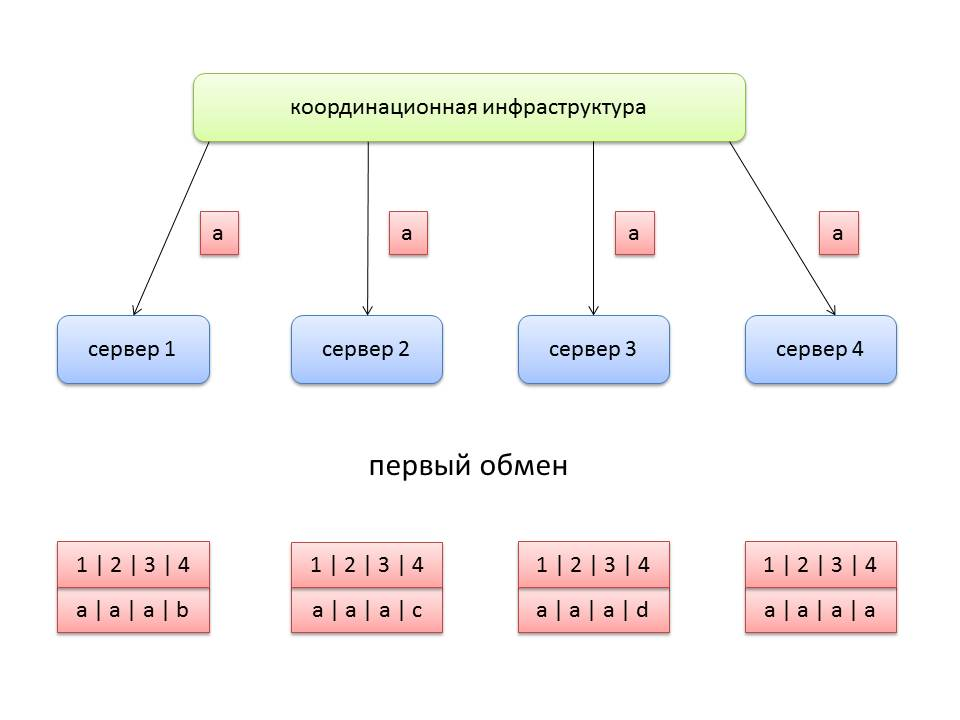
\includegraphics[width=0.8 \textwidth, height=0.6 \textwidth]{img/paxos1}  \caption{Алгоритм Paxos (1 этап)} \label{paxosjpg1}
\end{figure}
Это осуществляется при~помощи функции~\texttt{accept1(p, temp, server_port, tup)}, которая помещает полученные от~серверов значения в~соответствующий контейнер (полный программный код приведён в~\autocite{mybts}). 

Далее следует второй этап: серверы снова обмениваются полученными векторами друг с~другом, в~итоге у~каждого сервера имеется матрица утверждённых значений, как показано на~рисунке~\ref{paxosjpg2}. Данные манипуляции реализованы при~помощи функции~\texttt{accept2(p, temp, server_port, tup_dict)} (полный программный код приведён в~\autocite{mybts}).
\begin{figure}
	\centering 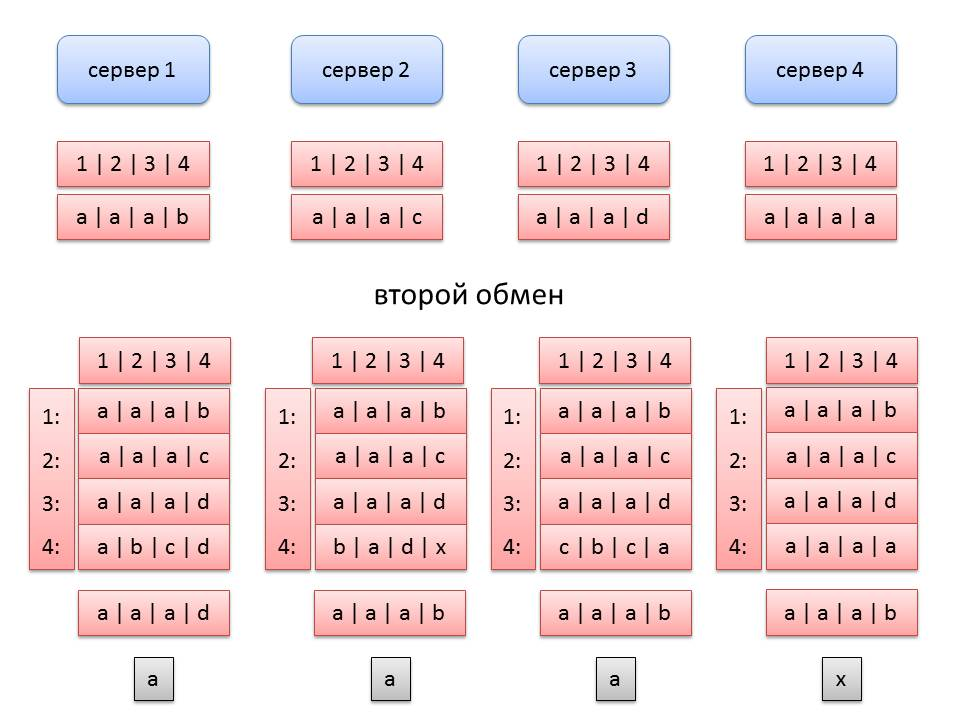
\includegraphics[width=0.8 \textwidth, height=0.6 \textwidth]{img/paxos2}  \caption{Алгоритм Paxos (2 этап)} \label{paxosjpg2}
\end{figure}
Далее в~каждом столбце матрицы выбирается наиболее часто встречающееся значение, оно помещается в~результирующий вектор. В~результирующем векторе снова находится значение, которое встречается чаще остальных. Это значение является утверждённым на~втором этапе. Таким образом Акцепторами принимается решение. Поскольку все сервера являются и Акцепторами, и Учениками, они уже знают, какое решение было принято, единственный Ученик, который не~знает о~принятом решении, это инфраструктура, поэтому ей отправляется сообщение о~том, какой кортеж был удалён из~пространства кортежей.

После~завершения работы функции~\texttt{paxos} возвращённое ею значение удаляется из~пространства кортежей. Происходит локальное освобождение ресурса при~помощи функции~\texttt{exit_r(temp, pid=None)}, удаляющей соответствующий запрос из~очереди (полный программный код приведён в~\autocite{mybts}). На~этом этапе завершается исполнение функции~\texttt{inp}.


\section{Полученные результаты}\label{sec:3}

\Conc

\printbibliography[heading=bibintoc]



\if 0
\begin{algorithm}[H]
	\caption{Операция out}\label{alg1}
	\begin{algorithmic}[1]
		\Statex $\{$client $p \}$
		\Procedure{out}{$t$}
		\ForAll {$s \in Q_w$}
		\State \Call{send}{$s, \langle$ OUT, $t \rangle$}
		\EndFor
		\EndProcedure
	\end{algorithmic}
\end{algorithm}
\begin{algorithm}[H]
	\caption{Операция out}\label{alg2}
	\begin{algorithmic}[1]
		\Statex $\{$server $s \}$
		\Upon{receive}{$p, \langle$ OUT, $t \rangle$}
		\If{$t \notin R_s$}
		\State $T_s \gets T_s \cup \{t\}$
		\EndIf
		\State $R_s \gets R_s \setminus \{t\}$
		\EndUpon
	\end{algorithmic}
\end{algorithm}

\begin{algorithm}[H]
	\caption{Операция rd}\label{alg3}
	\begin{algorithmic}[1]
		\Statex $\{$client $p \}$
		\Function{rdp}{$\bar t$}
		\State $T[s_1, \dots, s_n] \gets (\perp, \dots, \perp)$
		
		\ForAll {$s \in U$}
		\State \Call{send}{$s, \langle$ RD, $\bar t \rangle$}
		\EndFor
		
		\Repeat
		\State \Wait{receive}{$s, \langle$ TS, $T_s^{\bar t} \rangle$}
		\State $T[s] \gets T_s^{\bar t}$
		\Until{$\{s \in U$ : $T[s] \ne \perp \} \in \mathcal{Q}_r$}
		
		\If{$\exists t$ : ($|s$ : $t \in T[s]| \geqslant f + 1$)}
		\State \Return{$t$}
		\EndIf
		\State \Return{$\perp$}
		\EndFunction
	\end{algorithmic}
\end{algorithm}
\begin{algorithm}[H]
	\caption{Операция rd}\label{alg4}
	\begin{algorithmic}[1]
		\Statex $\{$server $s \}$
		\Upon{receive}{$p, \langle$ RD, $t \rangle$}
		\State $T_s^{\bar t} \gets \{t \in T_s$ : $match(t, \bar t)\}$
		\State send(p, $\langle$ TS, $T_s^{\bar t}\rangle$)
		\EndUpon
	\end{algorithmic}
\end{algorithm}

\begin{algorithm}[H]
	\caption{Операция in}\label{alg5}
	\begin{algorithmic}[1]
		\Statex $\{$client $p \}$
		\Function{in}{$\bar t$}
		\Repeat
		\State $t \gets$ \Call{enter}{rd($\bar t$)}
		\If{$t = \perp$}
		\State \Call{exit}{$\bar t$}
		\State \Return{$\perp$}
		\EndIf
		\State $d \gets$ \Call{paxos}{$p, t$}
		\Until{$d = t$}
		\State \Return{$t$}
		\EndFunction
	\end{algorithmic}
\end{algorithm}
\begin{algorithm}[H]
	\caption{Операция enter}\label{alg9}
	\begin{algorithmic}[1]
		\Statex $\{$client $p \}$
		\Function{enter}{$\bar t$}
		\State $T[s_1, \dots, s_{|Q_r|}] \gets (\perp, \dots, \perp)$
		
		\ForAll {$s \in U$}
		\State \Call{send}{$s, \langle$ ENTER, $p, \bar t \rangle$}
		\State $T[s] \gets T_s^{\bar t}$
		\EndFor
		
		\ForAll {$s \in Q_r$}
		\State \Wait{receive}{$s, \langle$ GO, $p, T_s^{\bar t} \rangle$}
		\State $T[s] \gets T_s^{\bar t}$
		\EndFor
		
		\If{$\exists t$ : ($|s$ : $t \in T[s]| \geqslant f + 1$)}
		\State \Return{$t$}
		\EndIf
		\State \Return{$\perp$}
		\EndFunction
	\end{algorithmic}
\end{algorithm}
\begin{algorithm}[H]
	\caption{Операция exit}\label{alg10}
	\begin{algorithmic}[1]
		\Statex $\{$client $p \}$
		\Procedure{exit}{$\bar t$}
		\ForAll {$s \in U$}
		\State \Wait{send}{$s, \langle$ EXIT, $p, \bar t \rangle$}
		\EndFor
		\EndProcedure
	\end{algorithmic}
\end{algorithm}

\begin{algorithm}[H]
	\caption{Операция enter}\label{alg6}
	\begin{algorithmic}[1]
		\Statex $\{$server $s \}$
		\Upon{receive}{$\langle$ ENTER $, p, \bar t \rangle$}
		\State $q_{\bar t} \gets $ \Call{append}{$q_{\bar t}, p$}
		\If{head($q_{\bar t}$) $ = p$}
		\State \Call{send}{$p, \langle$ GO $, $ rd($\bar t$) $\rangle$}
		\EndIf
		\EndUpon
	\end{algorithmic}
\end{algorithm}
\begin{algorithm}[H]
	\caption{Операция in}\label{alg7}
	\begin{algorithmic}[1]
		\Statex $\{$server $s \}$
		\Upon{receive}{$p, \langle$ IN $\bar t, t \rangle$}
		\State $d \gets $ \Call{paxos}{$\bar t, t$}
		\If{$d \ne \perp$}
		\If{$d \notin T_s$}
		\State $R_s \gets R_s \cup \{d\}$
		\EndIf
		\State $T_s \gets T_s \setminus \{d\}$
		\EndIf
		\State \Call{exit}{$p, type(\bar t)$}
		\EndUpon
	\end{algorithmic}
\end{algorithm}
\begin{algorithm}[H]
	\caption{Операция exit}\label{alg8}
	\begin{algorithmic}[1]
		\Statex $\{$server $s \}$
		\Upon{receive}{$p, \langle$ EXIT $, \bar t \rangle$}
		\State $q_{\bar t} \gets $ \Call{append}{$q_{\bar t}, p$}
		\If{head($q_{\bar t}$) $ = p$}
		\State $q_{\bar t} \gets $ \Call{tail}{$q_{\bar t}$}
		\If{$\neg$ \Call{empty}{$q_{\bar t}$}}
		\State \Call{send}{head($q_{\bar t}$), $\langle$ GO $, \bar t \rangle$}
		\EndIf
		\EndIf
		\EndUpon
	\end{algorithmic}
\end{algorithm}
\fi

\if 0
\section{Несколько примеров в~\LaTeX{}}
\label{sec:examples}
\subsection{Как оформить таблицу}
Для таблиц обычно используются окружения table и tabular --- см. таблицу~\ref{tab:widgets}. Внутри окружения tabular используются специальные команды пакета booktabs — они очень красивые; самое главное: использование вертикальных линеек считается моветоном.
\begin{table}
\centering
\caption{\label{tab:widgets}Подпись к таблице --- сверху}
\begin{tabular}{llr}
\toprule
\multicolumn{2}{c}{Item} \\
\cmidrule(r){1-2}
Животное  & Описание    & Цена (\$) \\
\midrule
Gnat      & per gram    & 13.65      \\
          & each        & 0.01       \\
Gnu       & stuffed     & 92.50      \\
Emu       & stuffed     & 33.33      \\
Armadillo & frozen      & 8.99       \\
\bottomrule
\end{tabular}
\end{table}

\fi

\end{document}
